\newpage
\section{Teoria}
\subsection{Filtros ativos}
Filtros ativos utilizam elementos amplificadores (transistores, amplificadores operacionais, etc.) em conjunto com resistores e capacitores para apresentar as características de filtragem desejadas.
Este tipo de filtro pode apresentar uma impedância de entrada alta, uma impedância de saída baixa e um ganho muito grande, tornando-os ideais para aplicações onde o sinal possui baixa potência. Porém sua principal característica é que não à necessidade de utilizar indutores para filtros de ordem maior, reduzindo o custo, tamanho e a falta de precisão características dos indutores.
O desempenho dos filtros ativos em altas frequências é limitado pelo ganho do circuito, quanto maior o ganho, menor a largura de banda disponível.
Filtros ativos também geram ruídos, devido ao elemento de amplificação, porém esses efeitos podem ser minimizados com o uso de amplificadores 	\textit{low noise} e técnicas de design apropriadas.

\subsection{Topologia Sallen-Key}
A figura \ref{f_skey} mostra uma das topologias mais utilizadas de filtros ativos. Esse é um filtro FPB Sallen-Key de segunda ordem, o qual pode ser utilizado com cascata para a obtenção de filtros de ordem maior.
Neste filtro, os dois resistores e os dois capacitores conectados a entrada não inversora definem a frequência de corte do mesmo e o fator Q. Os resistores da entrada inversora definem o ganho de tensão e também o fator Q. Assim, para um determinado fator Q, o ganho e a frequência não podem ser modificados de forma independente.

\begin{figure}[H]
\centering
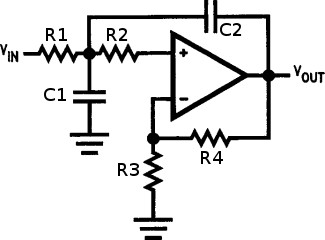
\includegraphics[scale=0.5]{Imagens/skey.jpg}
\label{f_skey}
\caption{Filtro ativo passa-baixas com topologia Sallen-Key.}
\end{figure}

\subsection{Ganho, frequência de corte e fator Q para FPB Sallen-Key}
O ganho é dado pelo divisor resistivo composto pelos resistores R3 e R4. A equação para o calculo do ganho é dada na eq. \ref{e_ganho}.

\begin{equation}
G = \frac{R3+R4}{R3} \quad [Volt/Volt].
\label{e_ganho}
\end{equation}

A frequência de corte é dada pela equação \ref{e_fc}.

\begin{equation}
f_c = \frac{1}{2\pi\sqrt{R1R2C1C2}} \quad [Hz]. 
\label{e_fc}
\end{equation}

E o fator Q pela equação \ref{e_Q}.

\begin{equation}
Q = \frac{\sqrt{R1R2C1C2}}{R1C1 + R2C1 + R1C2(1-\frac{R3+R4}{R3})}
\label{e_Q}
\end{equation}

\subsection{Largura de banda dos filtros ativos}
A frequência de corte ($f_c$ é a frequência para qual o filtro apresentará uma atenuação de 3dB e é o parâmetro fundamental para o projeto de filtros.
Outro parâmetro importante para os filtros do tipo passa-faixa e rejeita-faixa é a largura da banda de passagem, a qual é composta por uma frequência de corte inferior (denominada $f_1$) e uma superior ($f_2$). Para os filtros ativos, a largura de banda do sinal deve ser menor que a largura de banda do componente amplificador, a um ganho constante, para evitar a distorção do sinal.

